\documentclass[11pt,envcountsect,aspectratio=169]{beamer} %handout pour polycopier, draft pour le brouillon
% \usetheme[secheader]{Boadilla}
\usetheme{Nogent}
\usepackage[utf8]{inputenc}
\usepackage[french]{babel}
\usepackage[T1]{fontenc}
\usepackage{amsmath}
\usepackage{amsfonts}
\usepackage{amssymb}
\usepackage{pgf,tikz}
\usepackage[ruled,french]{algorithm2e}
\usepackage{multicol}

\author[Thomas S. \& Romain V.]{Thomas Saigre \& Romain Vallet}

\hypersetup{%
    bookmarksopen=false,
    pdfsubject={Projet optimisation M1 CSMI},
}





\newcommand{\frametitre}{\begin{frame}
    \begin{center}
    {\Large\bf \secname}
    \end{center}
    \end{frame}
}


\title{Résolution du problème isopérimétrique}
\subtitle{Projet optimisation \\ M1 CSMI \\ Université de Strasbourg}
%\setbeamercovered{transparent} 
%\setbeamertemplate{navigation symbols}{} 
%\logo{} 
%\institute{} 
\date{27 avril 2020}




% Macros
\newcommand{\R}{\mathbb{R}}
\newcommand{\Z}{\mathbb{Z}}
\newcommand{\C}{\mathcal{C}}
\renewcommand{\d}{\mathsf{d}}
\renewcommand{\P}{\mathcal{P}}
\renewcommand{\phi}{\varphi}
\newcommand{\A}{\mathsf{Aire}}
\newcommand{\p}{\mathsf{Per}}
\newcommand{\IA}{\textsf{IA}}
\newcommand{\IP}{\textsf{IP}}
\renewcommand{\Im}{\mathrm{Im}}
\renewcommand{\ss}{\vspace*{\baselineskip}}

\definecolor{ttttff}{rgb}{0.2,0.2,1}
\definecolor{xdxdff}{rgb}{0.49,0.49,1}


\newcommand\thm[2]{%
    \begin{beamerboxesrounded}[upper=titreB,lower=texteB,shadow=true]{Théorème : #1}
        \it #2
    \end{beamerboxesrounded}
    \normalfont
}

\newcommand\defi[2]{%
    \begin{beamerboxesrounded}[upper=titreB,lower=texteB,shadow=true]{Définition : #1}
        \it #2
    \end{beamerboxesrounded}
    \normalfont
}

\begin{document}


\begin{frame}[plain]
\titlepage
\end{frame}


% Introduction
\section[Introduction]{Introduction}


% \frametitre


% Table de matières
\begin{frame}{Table des matières}
\tableofcontents[hideallsubsections]
\end{frame}




\section{Définition du problème isopérimétrique}

\begin{frame}{Problème isopérimétrique}

\begin{beamerboxesrounded}[upper=titreB,lower=texteB,shadow=true]{Definition}
        Un \emph{problème isopérimétrique} est un problème d'optimisation qui vise à trouver un domaine de $\R^2$ (plus d'autres conditions) qui maximise l'aire pour un périmètre constant :
        \[\max_{D \in \C} \A(D) \label{ia}\tag{\IA}\]
        Avec $\mathcal{C} = \{ D \text{ convexe borné de } \R^2, \p(D) = p_0 \}$ avec $p_0 \in \R_+$ une constante.
\end{beamerboxesrounded}

Nous pouvons rajouter des contraintes sur $\C$.

\end{frame}

\begin{frame}{Problème iso-aire}

\begin{beamerboxesrounded}[upper=titreB,lower=texteB,shadow=true]{Definition}
        Un \emph{problème iso-aire} est un problème d'optimisation qui vise à trouver un domaine de $\R^2$ (plus d'autres conditions) qui minimise le périmètre pour une aire constante :
        \[\min_{D \in \C} \p(D) \label{ip}\tag{\IP}\]
        Avec $\mathcal{C} = \{ D \text{ convexe borné de } \R^2, \A(D)=c \}$ avec $c \in R^+$ une constante.
\end{beamerboxesrounded}

Nous pouvons rajouter des contraintes sur $\C$.

\vspace{\baselineskip}
Les problèmes \emph{isopérimétrique} et \emph{iso-aire} sont \textbf{équivalents}.

\end{frame}








\section{Maximisation d'une surface à périmètre constant}



\begin{frame}{Maximisation d'une surface à périmètre constant}

\begin{beamerboxesrounded}[upper=titreB,lower=texteB,shadow=true]{Théorème}
        La solution du problème \emph{isopérimétrique} (ou \emph{iso-aire}) avec $p_0=2\pi$ sans condition est un cercle.
\end{beamerboxesrounded}
% \vspace{\baselineskip}


\begin{proof}[Démonstration : \emph{dans le cas d'un arc $\C^1$}]

\only<1>{%
    Pour prouver le théorème, on utilise la théorie de Fourier.

    On pose une fonction $z: [-\pi,\pi] \rightarrow \R^2$ de classe $C^1$ tel que $z(-\pi)=z(\pi)$, s'écrivant $z = \sum_{n \in \Z}{c_n e_n}$, où $e_n=s\mapsto e^{ins}$ avec $n\in\Z$ et $s\in[-\pi,\pi]$.

    Le but est de prouver que $z = c_0 + c_1 e_1$.

    On montre (par des calculs) : $A=\pi\sum_{n\in\Z}n|c_n|^2$, où $A$ désigne l'air du domaine délimité par $z$ ($\Gamma_z$).

    Comme le périmètre de $\Gamma_z$ vaut $2\pi$,
    $\sum_{n\in\Z}n^2|c_n|^2=\int_{-\pi}^\pi |z'(s)|\d s=2\pi$.
}
\only<2>{%
    Astuce magique : $n\leqslant n^2$ d'où $A = \pi \sum_{n\in \Z}{n|c_n|^2} \leqslant \pi \sum_{n\in \Z}{n^2|c_n|^2} = \pi$
    \ss

    Condition d'optimalité : $A\leqslant\pi$, et le cercle vérifie cette condition.
    \ss

    On introduit la \emph{déviation} $w(s)=z(s)-(c_0+c_1e^{is})$, et on montre que $\Vert w\Vert_{H^1}=0$ (avec la majoration $1+n^2\leqslant \frac{5}{2}(n^2-n)$ pour $n\neq 0,1$) : donc $z$ est un cercle.

}
\end{proof}
\end{frame}








\section{Le problème de Didon}


\subsection{Le problème}


\begin{frame}{Problème de la reine Didon}

    \begin{itemize}
        \item Les terres où elle pourra s'établir seront \og autant qu'il pourrait en tenir dans la peau d'un b\oe{}uf\fg{}
        \item Exemple de la ville de Cologne, au Moyen-Âge :
    \end{itemize}
    
    \begin{figure}
        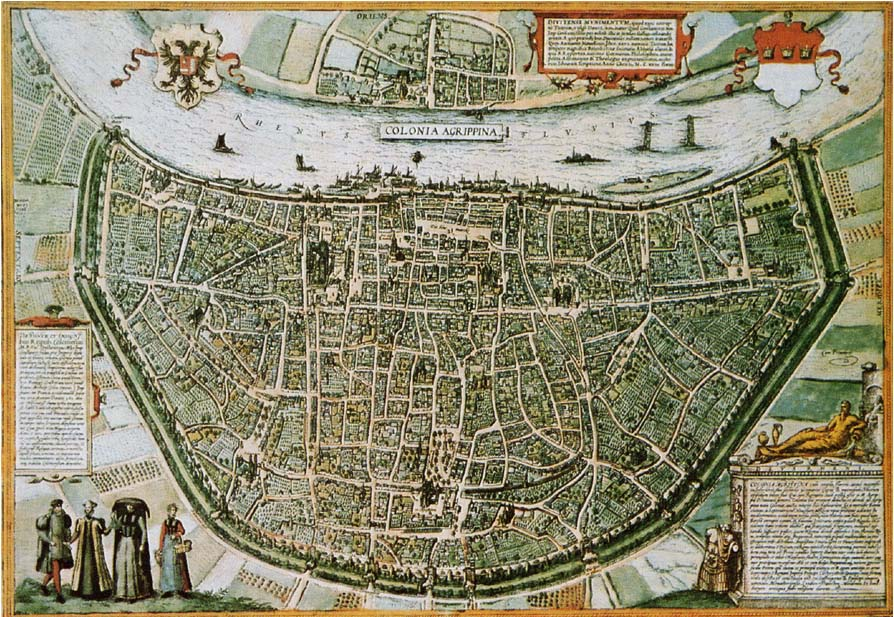
\includegraphics[scale=0.6]{img/cologne.jpg}
    \end{figure}

\end{frame}


\begin{frame}
    \frametitle{Position du problème}

    \begin{itemize}
        \item $\ell$ est fixé
        \item On cherche à maximiser l'aire du domaine pour un périmètre donné (ou de façon équivalente : minimiser le périmètre pour une aire donnée)
    \end{itemize}

    \begin{center}

        \begin{tikzpicture}
        \draw[->,color=black] (0,-0.5) -- (0,1);
        \fill[line width=0pt,color=ttttff,fill=ttttff,fill opacity=0.15] (-2,0) -- (2,0) -- (2,-0.5) -- (-2,-0.5) -- cycle;
        \begin{scriptsize}
        \fill [color=blue] (-2,0) circle (.5pt);
        \draw[color=blue] (-2,0) node[anchor=north] {$-\ell$};
        \fill [color=blue] (2,0) circle (.5pt);
        \draw[color=blue] (2.,0) node[anchor=north] {$+\ell$};
        \draw[color=black] (0,.8) node[anchor=south east] {$f$};
        \draw[color=ttttff] (0,-.5) node[anchor=south]{Mer};
        \end{scriptsize}
        \draw[smooth,samples=100,domain=-2.0:2.0] plot(\x,{0-((\x)-2)*((\x)+2)/5});
        \draw[->,color=black] (-2,0) -- (2,0);
        \end{tikzpicture}
        
        \end{center}

\end{frame}


\subsection{Résolution analytique}

\begin{frame}
    \frametitle{Résultat}

    \thm{}{%
        Le demi-cercle $y(x)=\sqrt{\ell^2-x^2}$ est solution du problème iso-aire en prenant $A_0=\frac{\pi}{2}\ell^2$. Il est donc solution du problème de Didon pour le choix de $p_0=\pi\ell$.
    }

    \begin{beamerboxesrounded}[upper=titreV,lower=texteV,shadow=true]{Rappel de cours (dimension infinie)}
        Un point critique d'un fonction differentiable convexe est un minimum.
    \end{beamerboxesrounded}



    \begin{proof}
    On montre que la fonction $y$ est un point critique de la fonction convexe $J\colon f\mapsto \int_{-\ell}^\ell \sqrt{1+f'(t)}\d t$. 
    à finir !!
    \end{proof}

\end{frame}





\subsection{Résolution numérique}

\begin{frame}
    \frametitle{Discrétisation}

    On discrétise en $n+2$ points $f_i = f(x_i)$ pour $i=-1,...,n$ ($f_{-1}=f_n=0$).

    \begin{beamerboxesrounded}[upper=titreB,lower=texteB,shadow=true]{Problème d'optimisation}
        Le problème devient un problème d'optimisation en dimension finie :
        \[\max_{f \in \left(\R^+\right)^n, \A(f)=a_0} lg(f)\]
        Avec :
        \begin{itemize}
            \item Aire : $\A(f) = h \sum_{i=0}^n{f_i}$
            \item Longueur : $lg(f) =  \sqrt{f_0^2+h^2} + \displaystyle\sum_{i=0}^{n-1}{\sqrt{\vphantom{f_n^2}{(f_{i+1}-f_i)}^2+h^2}} + \sqrt{f_{n-1}^2+h^2} $
        \end{itemize}
    \end{beamerboxesrounded}

\end{frame}

\begin{frame}
    \frametitle{Algorithme d'Uzawa}
    
    Nous allons utiliser l'algorithme d'Uzawa projeté (on effectue une projection pour voir un résultat positif, sans à ajouter de contrainte supplémentaire) :
    
    \begin{beamerboxesrounded}[upper=titreB,lower=texteB,shadow=true]{Formule du Lagrangien}
        Le Lagrangien s'écrit :
        \begin{eqnarray*}
            L \colon \R^n \times \R &\rightarrow & \R \\
            f, \lambda &\rightarrow & lg(f) + \lambda (\A(f)-a_0)
        \end{eqnarray*}
    \end{beamerboxesrounded}
    
    Mais au lieu de rechercher à chaque boucle $\min_{\rho} L(f_k - \rho \nabla L(f,\lambda))$ nous voulons juste : $L(f_{k+1}) = L(f_k - \rho \nabla L(f,\lambda)) < L(f_k)$.
    
    De même, nous ne voulons pas $\max_{\sigma} \lambda_k + \sigma (A(f)-a_0)$ mais juste : $\lambda_{k+1} = \lambda_k + \sigma (A(f)-a_0) > \lambda_k$.
    
    \ss

    Il s'agit d'une variante d'Uzawa (méthode d'Arrow--Huzwicz) : les étapes de recherches des \emph{min} et \emph{max} sont remplacées par des méthodes de gradient (montant ou descendant)

\end{frame}

\begin{frame}
    \frametitle{Présentation des algorithmes (1/3)}
    
    \begin{algorithm}[H]
    \caption{Résout le problème de Didon par Uzawa}
    \label{algo:didon}

        \KwIn{$f \in \R^n$ et $\lambda \in \R$}
        
        $f_0 \leftarrow f$
        
        $\lambda_0 \leftarrow \lambda$
        
        \While {condition d'arrêt}{
        $\rho_{k+1} \leftarrow \text{recherche\_rho($f_k$, $\lambda_k$)}$
        
        $f_{k+1} \leftarrow f_k - \rho_{k+1} Grad(f,\lambda)$
        
        projeter $f_{k+1}$ sur $(\R^+)^n$
        
        $\sigma_{k+1} \leftarrow \text{recherche\_sigma($f_{k+1}$, $\lambda_k$)}$
        
        $\lambda_{k+1} \leftarrow \lambda_k + \sigma_{k+1} (A(f_{k})-a_0)$
        
        $k \leftarrow k+1$
        }
        \KwOut f
 
    \end{algorithm}

\end{frame}

\begin{frame}
    \frametitle{Présentation des algorithmes (2/3)}
    
    \begin{algorithm}[H]
    \caption{recherche\_rho : Renvoie le pas pseudo-optimal pour la variable primale}
    \label{algo:primale}

        \KwIn{$f \in \R^n$ et $\lambda \in \R$}
        
        \KwResult{$L(fbis,\lambda) < L(f,\lambda)$ avec $fbis = f - \rho_i \nabla L(f,\lambda)$}

        $fbis_0 \leftarrow f$

        $\rho_0 = 1$ (valeur arbitraire)

        \While{$L(fbis_{i},\lambda) > L(fbis_{i-1},\lambda)$}{
            $\rho_{i+1} \leftarrow \rho_i / 1.2$

            $fbis_{i+1} \leftarrow fbis_i - \rho_{i+1} Grad(f,\lambda)$

            $i \leftarrow i+1$

        }
        \KwOut{$\rho_i$}

    \end{algorithm} 

\end{frame}


\begin{frame}
    \frametitle{Présentation des algorithmes (3/3)}   
    
    \begin{algorithm}[H]
        \caption{recherche\_sigma : Renvoie le pas pseudo-optimal pour la variable duale}
        \label{algo:duale}
    
        \KwIn{$f \in \R^n$ et $\lambda \in \R$}
        
        \KwResult{$\lambda bis > \lambda$ avec $\lambda bis = \lambda + \sigma (A(f)-a_0)$}
        $\lambda bis_0 = \lambda$

        $\sigma_0 \leftarrow 1$ (valeur arbitraire)

        \While{$\lambda bis_i < \lambda bis_{i-1}$}{
            $\sigma_{i+1} \leftarrow \sigma_i / 1.3$

            $\lambda bis_{i+1} \leftarrow \lambda bis_i + \sigma_{i+1} (A(f)-a_0)$

            $i \leftarrow i+1$
        }
        \KwOut{$\sigma_i$}
    
    \end{algorithm}
    
\end{frame}

\subsection{Résultats}

\begin{frame}
    \frametitle{Résultats}

    Avec $\ell=1$ et $a_0=\frac{\pi}{2}$ : la solution exacte est un demi-cercle.

    \begin{center}
    \def\echelle{0.3}
    \only<1>{%
        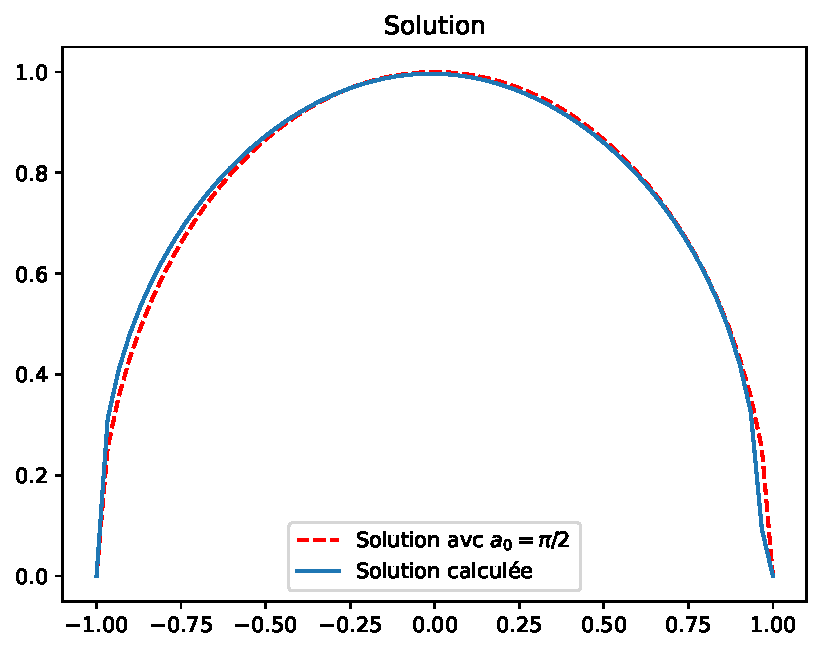
\includegraphics[scale=0.5]{../res/test_sol}
        \flushleft{Résultat obtenu : 3.1490304292815354}
    }
    \only<2>{%
        \flushleft{Évolution au cours des 980 itérations :}

        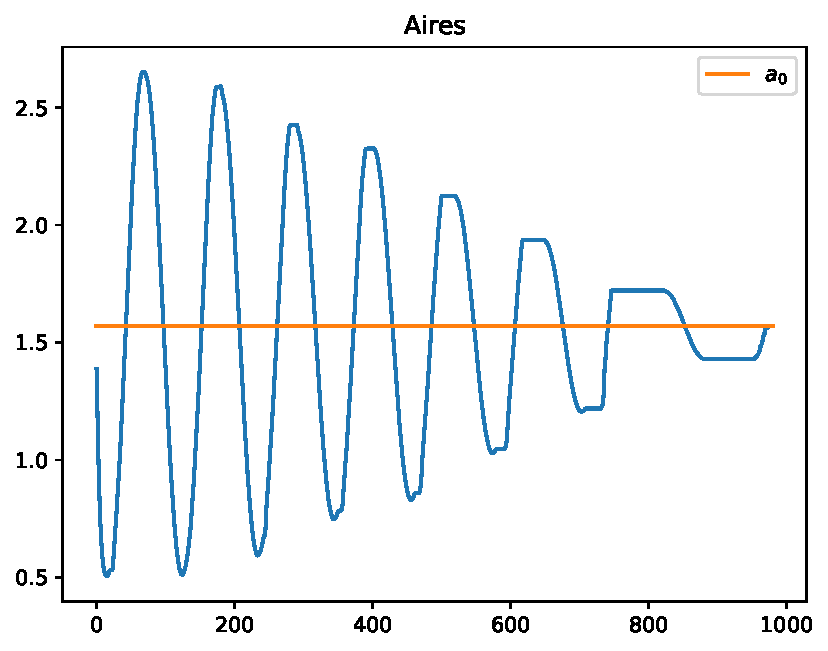
\includegraphics[scale=\echelle]{../res/test_aires}
        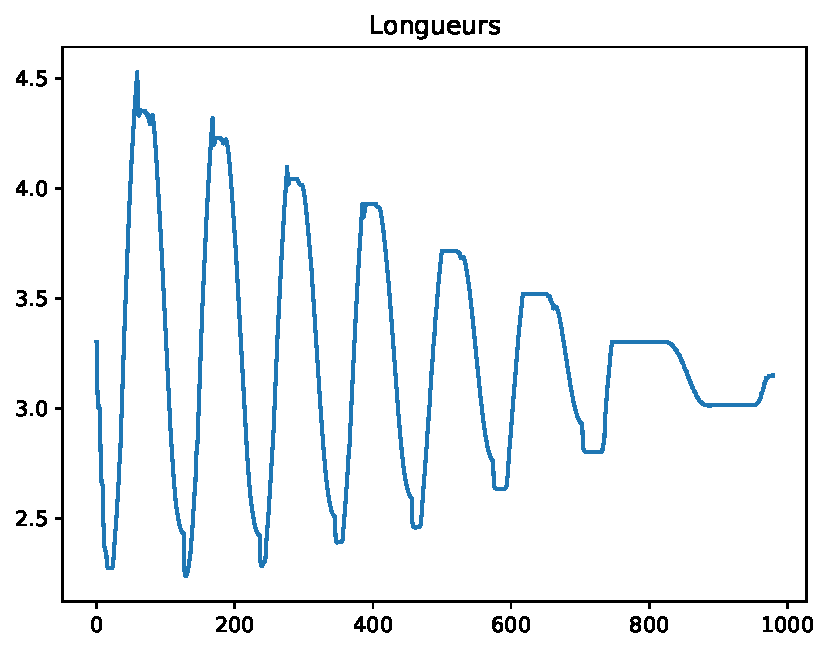
\includegraphics[scale=\echelle]{../res/test_longueurs}
        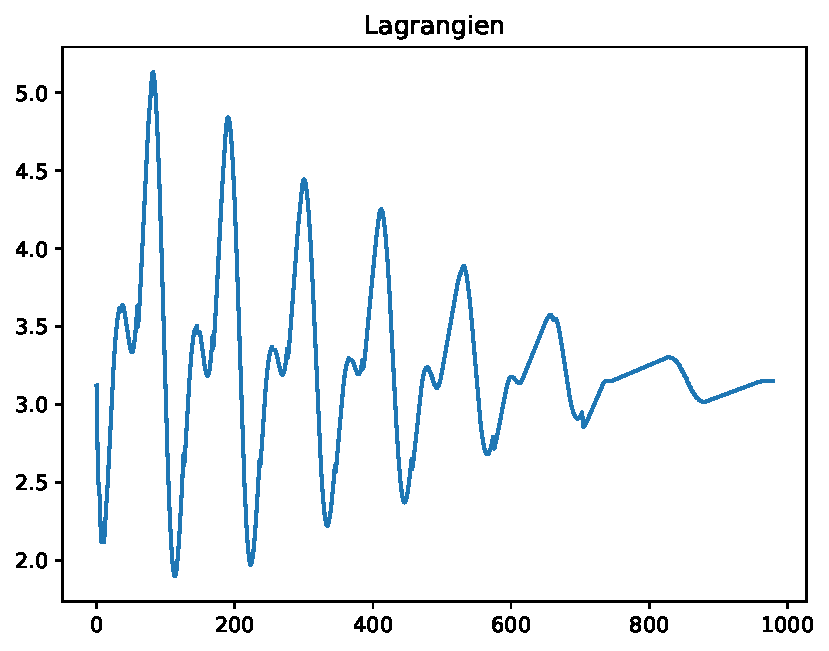
\includegraphics[scale=\echelle]{../res/test_lagrangien}
    }

    \end{center}

    

\end{frame}


\begin{frame}
\frametitle{Résultats (suite)}

\begin{center}

\begin{multicols}{2}
$a_0=1$
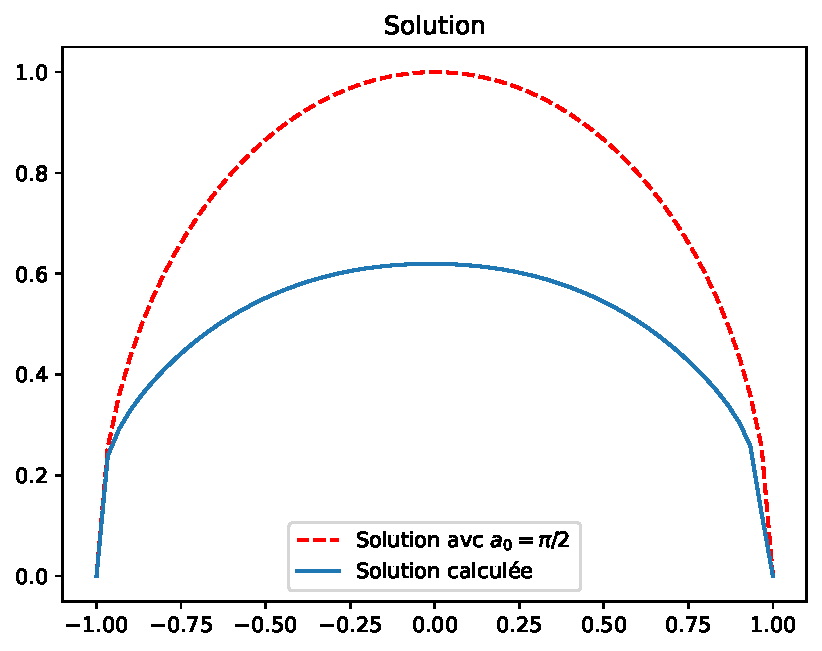
\includegraphics[scale=0.5]{../res/petit_sol}
En 287 itérations : 2.625

$a_0=3$
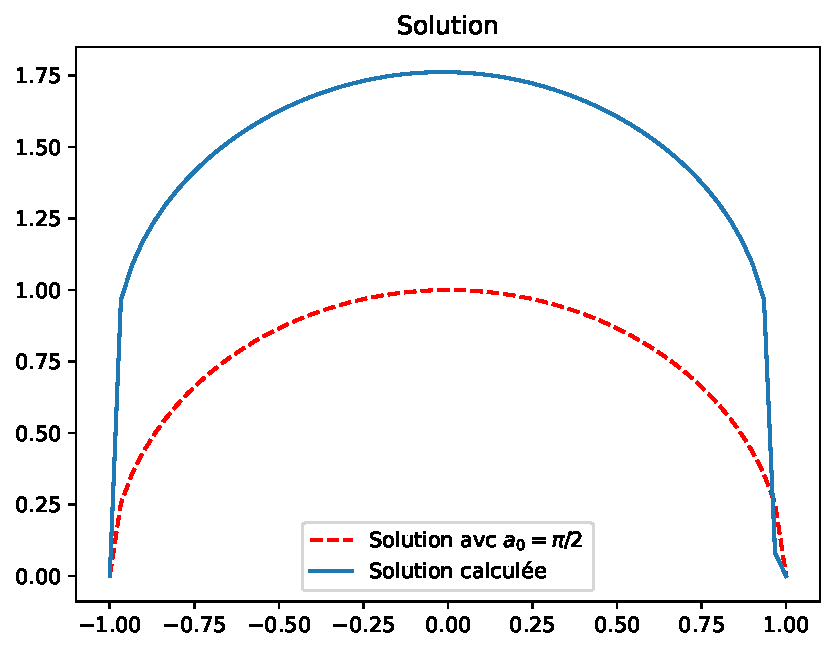
\includegraphics[scale=0.5]{../res/trois_sol}
En 2\,768 itérations : 4.622
\end{multicols}
\end{center}

\end{frame}


\subsection{Autres méthodes de résolution}

\begin{frame}
    \frametitle{Autre méthode de résolution : Lagrangien augmenté}

    \only<1>{%
    \begin{itemize}
        \item $L_b(f,\lambda)=lg(f) + \lambda\left(A(f)-a_0\right)+\dfrac{b}{2}\left(A(f)-a_0\right)^2$
        \item Mise à jour du multiplicateur : $\lambda^{n+1}=\lambda^n + b\left(A(f_k)-a_0\right)$

        \begin{center}
            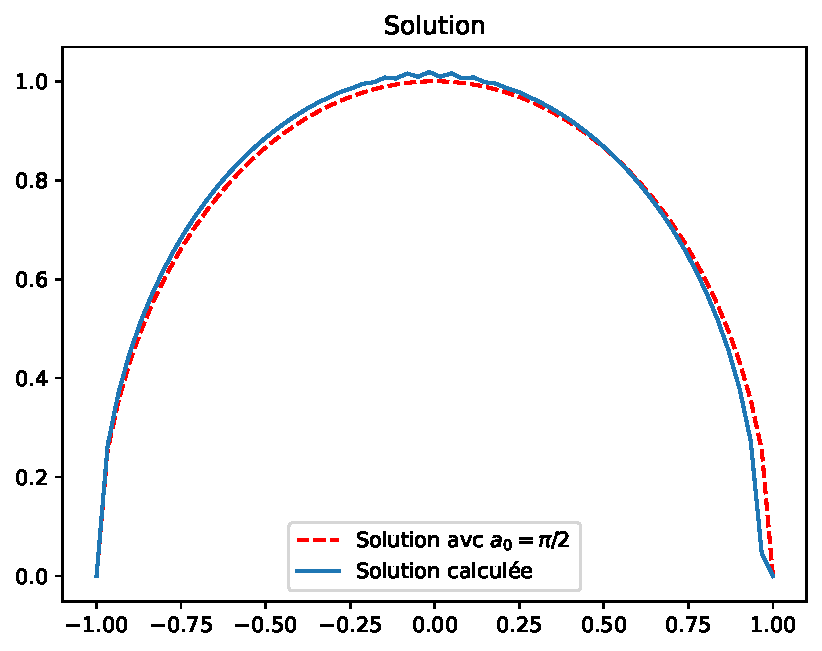
\includegraphics[scale=0.45]{../res/aug-pi_sol}

            $a_0=\frac{\pi}{2}$
        \end{center}
    \end{itemize}
    }

    \only<2>{%
    $a_0=4$, en 1\,671 itérations (contre au moins $2\times 10^5$ avec le lagrangien \og normal \fg{})
    \begin{center}
        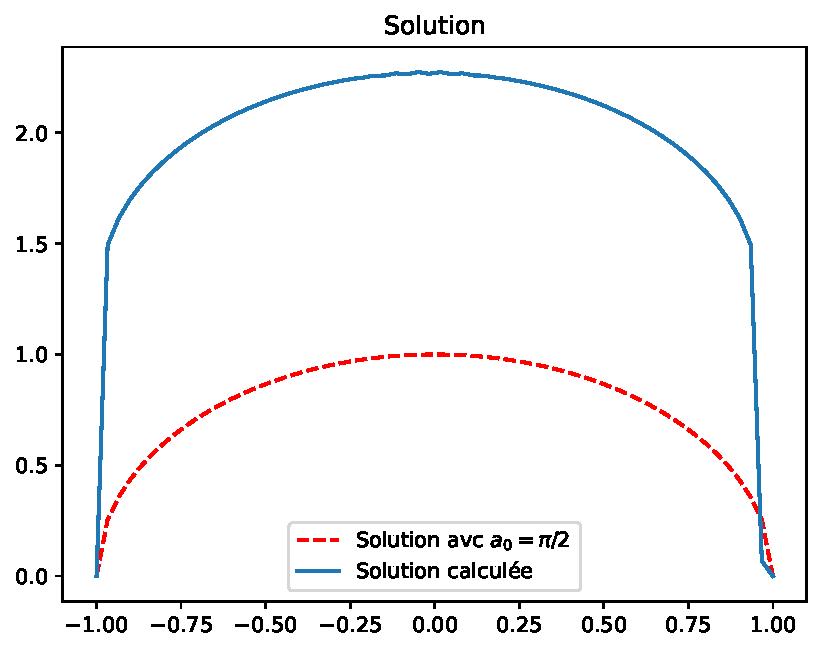
\includegraphics[scale=0.4]{../res/aug4_sol}
        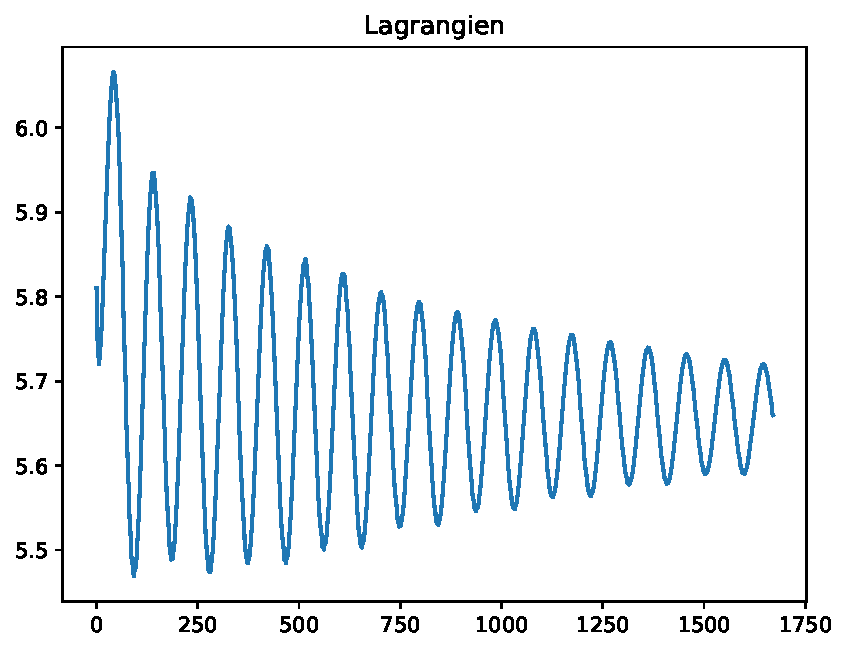
\includegraphics[scale=0.4]{../res/aug4_lagrangien}
    \end{center}
    }

\end{frame}





\end{document}